\documentclass{article}
\usepackage{../../../../format}
\lhead{A Level Maths - FP2}

%File specific Preamble

%Externalise to save computation time
\usetikzlibrary{external}
\tikzexternalize[prefix=tikz/]

%Give paragraphs the same format as sections
\setcounter{secnumdepth}{4}
\titleformat{\paragraph}
{\normalfont\normalsize\bfseries}{\theparagraph}{1em}{}
\titlespacing*{\paragraph}
{0pt}{3.25ex plus 1ex minus .2ex}{1.5ex plus .2ex}

\begin{document}
\begin{center}
\underline{\huge Polar Coordinates}
\end{center}
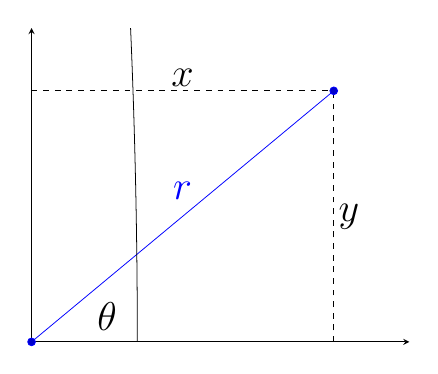
\begin{tikzpicture}[scale=0.7]
\begin{axis}[axis lines=middle,ymin=0,ymax=2.5,xmin=0,xmax=2.5,ticks=none]
\pgfplotsset{every tick label/.append style={font=\Huge}}

\addplot coordinates { (0,0) (2,2) };
\addplot [dashed] coordinates { (2,0) (2,2) };
\addplot [dashed] coordinates { (0,2) (2,2) };

\draw (axis cs: 0.7,0) arc[radius=70, start angle= 0, end angle= 45];
    \node[] at (axis cs: 0.5,0.2) {\huge $\theta$};
\node[blue] at (axis cs: 1,1.2) {\huge $r$};
\node[black] at (axis cs: 2.1,1) {\huge $y$};
\node[black] at (axis cs: 1,2.1) {\huge $x$};
\end{axis}
\end{tikzpicture}\\
Usual conventions are either $-\pi<\theta\leqslant\pi$ or $0\leqslant\theta<\pi$\\
\\
$x=r\cos\theta$\\
$y=r\sin\theta$\\
$r^2=x^2+y^2$\\
$\theta=\arctan\Big(\dfrac{y}{x}\Big)$
\section{Converting between polar and Cartesian form}
\subsection{Example 1}
\textit{Find the Cartesian equation of:}
$r=5$
$$\sqrt{x^2+y^2}=5$$
$$x^2+y^2=25$$
\subsection{Example 2}
\textit{Find the Cartesian equation of:}
$$r=2+\cos2\theta$$
Replace r and convert $\cos2\theta$
$$\sqrt{x^2+y^2}=2+\cos^2\theta-\sin^2\theta$$
Convert $\sin^2\theta$ and $\cos^2\theta$
$$\sqrt{x^2+y^2}=2+\frac{x^2}{x^2+y^2}-\frac{y^2}{x^2+y^2}$$
Multiply all terms by $x^2+y^2$
$$(x^2+y^2)^{\frac{3}{2}}=3x^2+y^2$$
\newpage
\section{Sketching polar curves}
To plot less standard types we look for axes intercepts and max and min values
\subsection{Standard types}
\subsubsection{r=a}
A circle, centre (0,0) with a radius of a
\subsubsection{$\theta=\alpha$}
A half line starting from (0,0) making an angle of $\alpha$ with the initial line (positive x axis)
\subsubsection{$r=a\theta$}
A spiral starting at the origin
\subsection{Cardioid type}
\subsubsection{$r=a(1+\cos\theta)$}
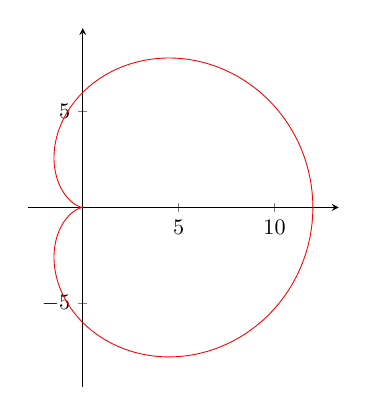
\begin{tikzpicture}[scale=0.8]
\begin{axis}[
    axis lines=center,
    axis equal image,
    enlargelimits=true,
     ]
    \addplot[data cs=polar,red,domain=0:360,samples=360,smooth] (x,{6*(1+cos(x))});
\end{axis}
\end{tikzpicture}
\subsubsection{$r=a(p+q\cos\theta)$}
\paragraph{p=q}
Factor out the value of p and plot as normal
\paragraph{$p\geqslant2q$}
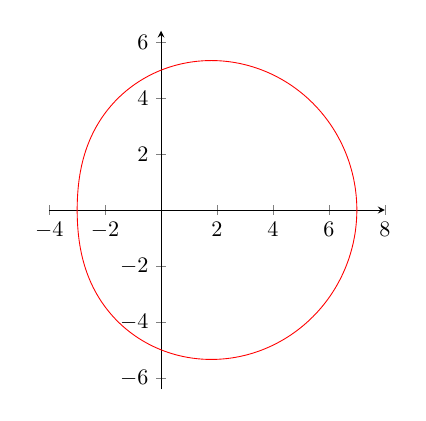
\begin{tikzpicture}[scale=0.8]
\begin{axis}[
    axis lines=center,
    axis equal image,
    enlargelimits=true,
     ]
    \addplot[data cs=polar,red,domain=0:360,samples=360,smooth] (x,{(5+2*cos(x))});
\end{axis}
\end{tikzpicture}
\newpage
\paragraph{$q\leqslant p<2q$}
\begin{tikzpicture}[scale=0.8]
\begin{axis}[
    axis lines=center,
    axis equal image,
    enlargelimits=true,
     ]
    \addplot[data cs=polar,red,domain=0:360,samples=360,smooth] (x,{(3+2*cos(x))});
\end{axis}
\end{tikzpicture}
\subsubsection{$r^2=a^2\cos2\theta$}
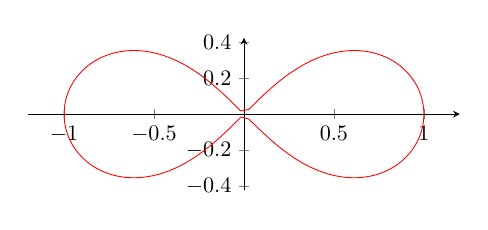
\begin{tikzpicture}[scale=0.8]
\begin{axis}[
    axis lines=center,
    axis equal image,
    enlargelimits=true,
     ]
    \addplot[data cs=polar,red,domain=0:360,samples=8000] (x,{sqrt(cos(2*x))});
\end{axis}
\end{tikzpicture}
\\
The 4 asymptotes are half lines at $\theta=\frac{\pi}{4},\frac{3\pi}{4},\frac{5\pi}{4},\frac{7\pi}{4}$
\subsection{$r^2=a^2\sin2\theta$}
\begin{tikzpicture}[scale=0.8]
\begin{axis}[
    axis lines=center,
    axis equal image,
    enlargelimits=true,
     ]
    \addplot[data cs=polar,red,domain=0:360,samples=8000] (x,{sqrt(sin(2*x))});
\end{axis}
\end{tikzpicture}
\\
This is an anticlockwise rotation of $r^2=a^2\cos2\theta$ by $\frac{\pi}{4}$, it is this not $\frac{\pi}{2}$ as the phase difference between $\cos2\theta$ and $\sin2\theta$ is $\frac{\pi}{4}$ compared to $\frac{\pi}{2}$ with one $\theta$.
\subsubsection{$r=a(p+q\sin\theta)$}
\begin{tikzpicture}[scale=0.8]
\begin{axis}[
    axis lines=center,
    axis equal image,
    enlargelimits=true,
    ticks=none
     ]
    \addplot[data cs=polar,red,domain=0:360,samples=360,smooth] (x,{6*(1+sin(x))});
\end{axis}
\end{tikzpicture}
\\
This is a rotation of $r=a(p+q\cos\theta)$ anticlockwise by $\frac{\pi}{2}$
\subsection{Other types}
\subsubsection{$r=a\sin3\theta$}
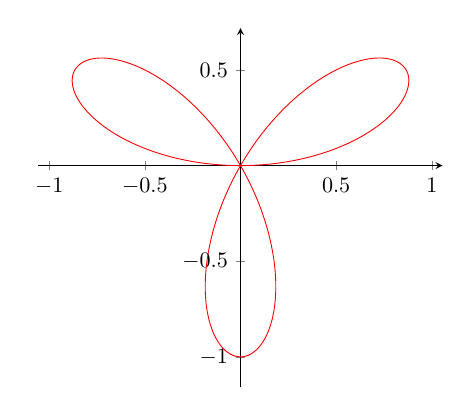
\begin{tikzpicture}[scale=0.8]
\begin{axis}[
    axis lines=center,
    axis equal image,
    enlargelimits=true,
     ]
    \addplot[data cs=polar,red,domain=0:360,samples=360,smooth] (x,{sin(3*x)});
\end{axis}
\end{tikzpicture}
\\
Asymptotes occur when $r=0$
\subsubsection{$r=2\sec(\theta-\frac{\pi}{3})$}
\begin{tikzpicture}[scale=0.8]
\begin{axis}[
    axis lines=center,
     ]
    \addplot[data cs=polar,red,domain=-10:100,samples=360,smooth] (x,{2/(cos(x-60))});
\end{axis}
\end{tikzpicture}
\newpage
\section{Integration}
$$\textrm{Area}=\frac{1}{2}\int^\beta_\alpha r^2 \ d\theta$$
Where the area of the sector is bounded by the half lines $\theta=\alpha$ and $\theta=\beta$, the value of $\theta$ must always be in radians.\\
\\
The the radius in this sector must not drop to zero, choose angles so this doesn't happen. Or choose multiple sections and add together, or use symmetry. 
\section{Differentiating Polar Equations to find tangents}
We only find tangents parallel and perpendicular to the initial line.\\
\\
$x=r\cos\theta$\\
$y=r\sin\theta$\\
\\
Using the chain rule:
$$\frac{dy}{dx}=\frac{dy}{d\theta}\times\frac{d\theta}{dx}$$
\\
Parallel: $\frac{dy}{d\theta}=0$\\
Perpendicular: $\frac{dx}{d\theta}=0$
\subsection{Example}
$r=a(1+\cos\theta)$\\
\\
Find the coordinates where the tangents are parallel to the initial line with $\theta=0$\\
\\
$$y=r\sin\theta$$
\textcolor{red}{Replace r with $a(1+\cos\theta)$}
$$y=a(\sin\theta+\sin\theta\cos\theta)$$
\textcolor{red}{Now we can find $\frac{dy}{d\theta}$}
$$\frac{dy}{d\theta}=a(\cos\theta+\cos^2\theta-\sin^2\theta)$$
\textcolor{red}{Simplify and set equal to zero}
$$2\cos^2\theta+\cos\theta-1$$
$$0=(2\cos\theta-1)(\cos\theta+1)$$
\textcolor{red}{Find $\cos\theta$, $\theta$ and $r$}
$$\cos\theta \quad \cos\theta=-1$$
$$\theta=\pm\frac{\pi}{3} \quad \theta=\pi$$
$$r=\frac{3a}{2} \quad r=0$$
\subsubsection{Finding the equations of tangents}
$$\textrm{Cartesian equation:} \ y=r\sin\theta$$
$$\textrm{Polar equation:} \ r=y\csc\theta=r\sin\theta\csc\theta$$

\end{document}
